%        File: hw1.tex
%     Created: Sat Apr 06 10:00 AM 2013 P
% Last Change: Sat Apr 06 10:00 AM 2013 P
%
\documentclass[11pt]{article}

\usepackage{amsmath, amssymb, amsthm, cite, graphicx, float, mathrsfs, commath, dsfont, bbm, bm}
\usepackage[mathscr]{eucal}
\usepackage[sc]{mathpazo}
\linespread{1.05}
%\usepackage{setspace}
%\onehalfspacing
\usepackage[margin=1in, top=.8in, left=.8in]{geometry}
\usepackage{color}

% new commands
\DeclareMathOperator*{\argmin}{arg\,min}
\DeclareMathOperator{\sgn}{sgn}
\newcommand{\E}{\mathrm{E}}
\newcommand{\Var}{\mathrm{Var}}
\newcommand{\Cov}{\mathrm{Cov}}
\newcommand{\Cor}{\mathrm{Cor}}
\newcommand{\id}{\operatorname{id}}
\newcommand{\diag}{\operatorname{diag}}
\newcommand{\Id}{\operatorname{Id}}
\newcommand{\tr}{\operatorname{tr}}
\newcommand{\Q}{\mathbb{Q}}
\newcommand{\C}{\mathbb{C}}
\newcommand{\R}{\mathbb{R}}
\newcommand{\Z}{\mathbb{Z}}
\newcommand{\F}{\mathbb{F}}
\newcommand{\N}{\mathbb{N}}

\newcommand{\indep}{\rotatebox[origin=c]{90}{$\models$}}

% 524 commands
%\newcommand{\norm}[1]{\| #1 \|}
\DeclareMathOperator{\spn}{span}
%\newcommand{\spn}{\operatorname{span}}
\newcommand{\onenorm}[1]{\| #1 \|_{L^1(\mathbb R^d)}}
\newcommand{\twonorm}[1]{\| #1 \|_{L^2(\mathbb R^d)}}

% 534 commands
\renewcommand{\Re}{\text{Re\,}}
\renewcommand{\Im}{\text{Im\,}}

\begin{document}
\pagestyle{empty}
\hfill Abraham Engle

\hfill Stat 571

\hfill \today
\begin{enumerate}
 	%1
	\item 	
		\begin{enumerate}
		%a
		\item The fitted correlation between random slopes and random intercepts is $\approx 0.753>0$. 
		\\ \\First, the between-subject variability in reaction times appears to be quite large. The fitted standard deviations for the random effects are $(37.533077,5.922156)$ for intercept, slope respectively, compared to the fixed-effect standard errors $(9.049941,1.545793)$ also intercept, slope respectively.
		\\ \\ At the subject level, the positive correlation means we therefore associate larger intercepts (i.e., slower base-line reaction times) with larger slopes (steeper change in reaction time per day of sleep depravation). My answer would be unchanged if the magnitudes were not as large in the previous paragraph, but I think the larger between-subject variability makes me take this fitted correlation a bit more seriously.
		\item Both graphs are below:
		\begin{figure}[H]
			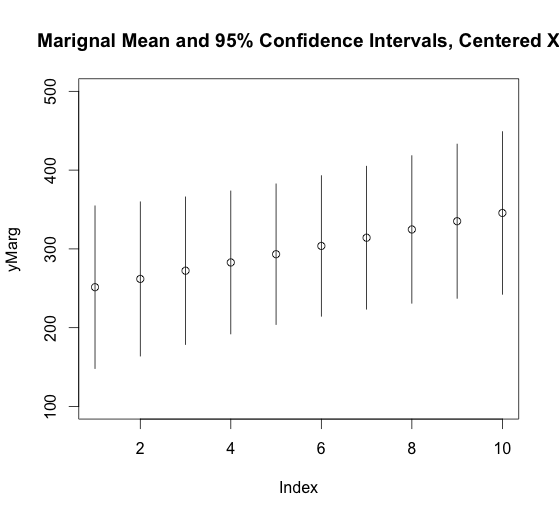
\includegraphics[scale=0.4]{Rplot1}
			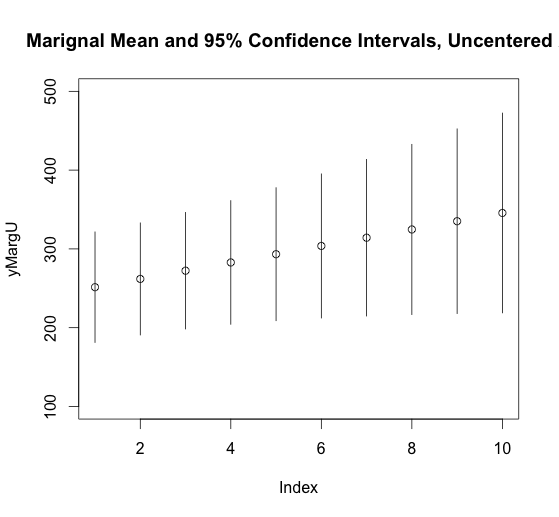
\includegraphics[scale=0.4]{Rplot2}
		\end{figure}
		By only changing the centering of the \texttt{Days} variable, the length of the 95\% confidence intervals changes, but the marginal fitted values (the centers of the bands) do not change. Depending on our research question about reaction time and its association to sleep depravation, we might desire narrower confidence intervals for smaller amounts of sleep depravation, which we see occurring in the uncentered case. In the uncentered case, our confidence bands fan out as sleep depravation increases. On the other hand, n the centeredi case, the bands fan out in both directions from the centering location, so I would prefer the centered \texttt{Days} variable.
		\end{enumerate}
	%2
	\item Setting $n=10^3, n_i=5$ for all $i=1,2,\dotsc,n$ and $\sigma_Y = 6, \sigma_b=1$, I generated data from the mechanism and fit a linear mixed model of the form $y_{ij} = \beta_0 + b_i + \epsilon_{ij}$. I obtained $\widetilde{b}_i$ for $i=1,2,\dotsc,n$ given on slide 3.62 using the ranef function and obtained $\widetilde{s}_i$ given by plug-in estimates of the conditional distribution of $b_i$ at the bottom of slide 3.61 via the se.ranef function.
	\\ Fixing the known $b_i, i=1,2,\dotsc,n$ and generating data as above, after $10^4$ replications using the same $b_i$ each time, I found the median of the proportions to be $95\%$ and the mean to be about $91.6\%$. The histogram of proportions over the $10^4$ replicates is
	\begin{figure}[H]
	\centering
		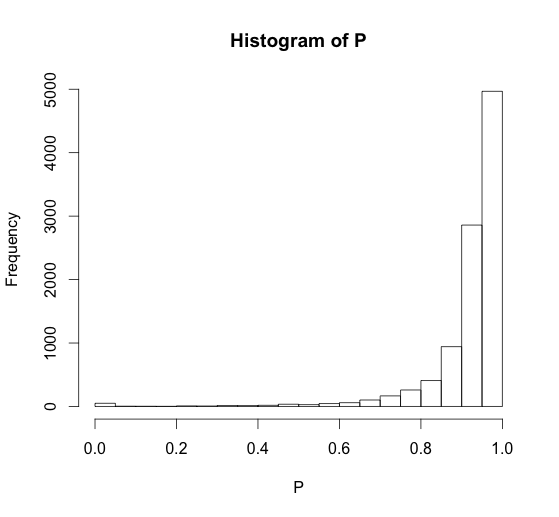
\includegraphics[scale=0.5]{Rplot3}
		\caption{10,000 replicates of data generating mechanism for $n=1000$ and $n_i=5$, and fixed, known $b_i$}
	\end{figure}
	The histogram exhibits skewness with fairly heavy tails, which explains the difference between the mean and median.
	%3
	\item
		\begin{enumerate}
			\item The marginal model for the $j$th observation is
			\[
				\log\left(\frac{E[Y_{ij}]}{1-E[Y_{ij}]} \right) = \gamma_0 + \gamma_1\texttt{gender}_{ij} + \gamma_2\texttt{hfora}_{ij} + \gamma_3\texttt{cos}_{ij} + \gamma_4\texttt{sin}_{ij} + \gamma_5\texttt{xero}_{ij} + \gamma_6\texttt{age}_{ij} + \gamma_7\texttt{age}^2_{ij}
			\]
			where $\texttt{sin}_{ij} = \sin\left(\frac{\pi(t+1)}{2}\right)$ and $\texttt{cos}_{ij} = \cos\left(\frac{\pi(t+1)}{2}\right)$ and where $t$ is time, measured in quarters.
			
			Before beginning the marginal interpretation, I want to deal with the trigonometric terms in two different ways. We can sine and cosine term into a single wave with different amplitude and phase:
			\[
				\gamma_3\cos\left(\frac{\pi(t+1)}{2}\right)+\gamma_4\sin\left(\frac{\pi(t+1)}{2}\right) = R\cos\left(\frac{\pi(t+1)}{2} - \delta \right),
			\]
			where $R = \sqrt{\gamma_3^2+\gamma_4^2}$ and where $\tan\delta = \gamma_4/\gamma_3$ and instead base parameter interpretations on controlling for the phase and amplitude of the above wave as a function of only the time variable. I provide this interpretation and the original interpretation, keeping in mind that our experiment only records times $t=1,2,\dotsc,6$.
			\begin{itemize}
				\item $\gamma_0$: log-odds of presence of respiratory infection for male children at height-for-age equal to zero (average height-for-age) without dry eye syndrome at \texttt{age} = 0 (average age) at time(s) given in terms of the displaced cosine wave:
				\[
					\frac{\pi(t+1)}{2} - \delta = (2k+1)\frac{\pi}{2}\Longrightarrow t = \frac{2}{\pi}\delta + 2k,\; k\in \Z.
				\]
				 Again, since the study only measures times at $t=1,2,\dotsc,6$, if none of those times actually satisfy the equation above (for any choice of $k$), the intercept interpretation is probably not very useful.
				\item $\gamma_1$: Log-odds ratio of infection between males and females controlling for all other covariate values.
				\item $\gamma_2$: Log-odds ratio of infection for a unit increase in height-for-age controlling for all other covariate values.
				\item $R$: Log-odds ratio of infection per time increase so that
				\[
					\cos\left(\frac{\pi(t+2)}{2} - \delta \right) - \cos\left(\frac{\pi(t+1)}{2} - \delta \right)= -\sqrt{2}\sin\left(\frac{\pi(3 + 2 t)}{4} -  \delta\right) = 1
				\]
				controlling for other covariates.
				\item $\delta$: This is the phase of the cosine wave we are using to model the time. Controlling for other covariates, the phase governs the link-transformed marginal mean masked through the cosine term.
				\item $\gamma_5$: Log-odds ratio of infection between those without dry eye and those with dry eye controlling for all other covariate values.
				\item $\gamma_6,\gamma_7$: Controlling for all other covariates, these terms govern the quadratic relationship between the link-transformed mean function and age. For example, $\gamma_7>0$ stipulates a convex quadratic.
			\end{itemize}
			Alternatively, we could instead try to interpret the values of $\gamma_3$ and $\gamma_4$ simultaneously, since they depend on the same covariate. We know the time values in our study, and a table displaying the possibilities of the cosine and sine waves is
			\begin{table}[H]
			\centering
				\begin{tabular}{c|r|r}
					$t$ & \texttt{cos} & \texttt{sin} \\
					\hline
					1 & -1 & 0 \\
					2 & 0 & -1 \\
					3 & 1 & 0 \\
					4 & 0 & 1 \\
					5 & -1 & 0 \\
					6 & 0 & -1
				\end{tabular}
				\caption{Table of Possible Sine and Cosine Values for Observed Times}
			\end{table}
			Therefore we can say that $\gamma_3-\gamma_4$ is the log-odds ratio of infection when passing from $t=1$ to $t=2$ or from $t=5$ to $t=6$, controlling for other covariates. Similarly, $\gamma_3 + \gamma_4$ is the log-odds ratio of infection when passing from time $t=2$ to $t=3$, again controlling for other covariates. 
			\item The estimates from GEE are
			\begin{table}[H]
			\centering
				\begin{tabular}{l | r | r}
					& Est & SE \\
					\hline
				$\gamma_0$ & $-2.0521$ & 0.212 \\
				$\gamma_1$ & $-0.48240$ & 0.23940 \\
				$\gamma_2$ & $-0.0406$ & 0.02358\\
				$\gamma_3$ & $-0.5922$ & 0.17130\\
				$\gamma_4$ & $-0.1707$ & 0.14710\\
				$\gamma_5$ & $0.607$ & 0.41990\\
				$\gamma_6$ & $-0.3678$ & 0.09508\\
				$\gamma_7$ & $-0.1573$ & 0.06368\\
				\end{tabular}
				\caption{GEE Parameter Estimates and Standard Errors}
			\end{table}
			\item The conditional model for the $j$th observation of the $i$th child is
			\[
				\log\left(\frac{E[Y_{ij}]}{1-E[Y_{ij}]} \right) = b_i + \gamma_0 + \gamma_1\texttt{gender}_{ij} + \gamma_2\texttt{hfora}_{ij} + \gamma_3\texttt{cos}_{ij} + \gamma_4\texttt{sin}_{ij} + \gamma_5\texttt{xero}_{ij} + \gamma_6\texttt{age}_{ij} + \gamma_7\texttt{age}^2_{ij}
			\]
			\begin{itemize}
				\item $\gamma_0$: As before, if there are no times satisfying the equation, interpreting the intercept might not be useful. Otherwise, it is the log-odds of presence of respiratory infection for an average (so the random intercept is zero) male child at average height-for-age without dry eye syndrome at average age measured at time(s) given in (b). 
				\item $\gamma_1$: Log-odds ratio of infection between average males and average females (so $b_i=0$ in both cases) controlling for all other covariate values.
				\item $\gamma_2$: Log-odds ratio for infection for a unit increase in height-for-age for an average child, controlling for all other covariate values.
				\item $R, \delta$: Same as in (b) except only holding for an average child and controlling for other covariates.
				\item $\gamma_3, \gamma_4$: Same as in (b) except only holding for an average child and controlling for other covariates.
				\item $\gamma_5$: Log-odds ratio of infection between an average child without dry-eye and an average child with dry-eye  controlling for all other covariate values.
				\item $\gamma_6, \gamma_7$: Same as in (b) except only holding for an average child, so we keep the $b_i=0$, and as usual controlling for other covariates.
			\end{itemize}
			\item Running GLMM in R on the model in (c) using random intercepts and a warm start for the algorithm at the estimate obtained from GEE analysis in (b) [the algorithm terminated with a warning that $\norm{\nabla f} \approx 0.0016$, which I couldn't get much lower without using the nAGQ flag in addition to the warm-start like on slide 3.104], I found (using the \texttt{texreg} package for \LaTeX  output)
\begin{table}[H]
\begin{center}
\begin{tabular}{l c }
\hline
 & Model 1 \\
\hline
(Intercept)                     & $-2.29^{***}$ \\
                                & $(0.25)$      \\
sex                             & $-0.51^{*}$   \\
                                & $(0.26)$      \\
ht.for.age                      & $-0.05^{*}$   \\
                                & $(0.02)$      \\
cos                             & $-0.61^{***}$ \\
                                & $(0.17)$      \\
sin                             & $-0.16$       \\
                                & $(0.17)$      \\
xerop                           & $0.53$        \\
                                & $(0.49)$      \\
poly(age, degree = 2, raw = T)1 & $-0.37^{***}$ \\
                                & $(0.10)$      \\
poly(age, degree = 2, raw = T)2 & $-0.15^{**}$  \\
                                & $(0.06)$      \\
\hline
AIC                             & 678.51        \\
BIC                             & 724.32        \\
Log Likelihood                  & -330.26       \\
Num. obs.                       & 1200          \\
Num. groups: id                 & 275           \\
Var: id (Intercept)             & 0.65          \\
\hline
\multicolumn{2}{l}{\scriptsize{$^{***}p<0.001$, $^{**}p<0.01$, $^*p<0.05$}}
\end{tabular}
\caption{Statistical models}
\label{table:coefficients}
\end{center}
\end{table}
			and the random effect slope $b_i$ has a fitted standard deviation of $\sqrt{0.65} \approx 0.804$, a little over three times larger than the fixed effects standard error.
			%e
			\item From the GEE and GLMM analysis, the coefficient estimates are of the same order of magnitude and sign along with the standard errors from both models. The biggest change is in the estimate of \texttt{xerop}, where its coefficient estimate is smaller in the GLMM and has a larger standard error. In both models, the $p$-value reported is relatively large, 0.14 and 0.28 in GEE and GLMM, respectively, while other covariates all have smaller $p$-values. I think there is a mild association between dry eye syndrome and respiratory infection based off this data, but I think the other predictors appear to have an even greater association. In particular, it does appear that age has a significant association with respiratory infection in both models. \\ \\Both the linear and quadratic coefficient estimates are negative in each case, so marginally we should expect the probability of respiratory infection to decrease as age increases when controlling for all other covariates (in particular, controlling for time, so we cannot make within-subject statements). Conditionally, we can say the same thing except that we need to specify the statement holds for an average child.
		\end{enumerate}
	%4
	\item The problem only calls for mean model diagnostics, so I omit the  leave-one-out diagnostic plots addressing large $n$ validity and influence of a particular individual. I also omit the variance plots. I plot the Pearson subject-level residuals against subject-level fitted values and against the other seven covariates looking for violation of the mean model assumption. 
%	\begin{figure}
%		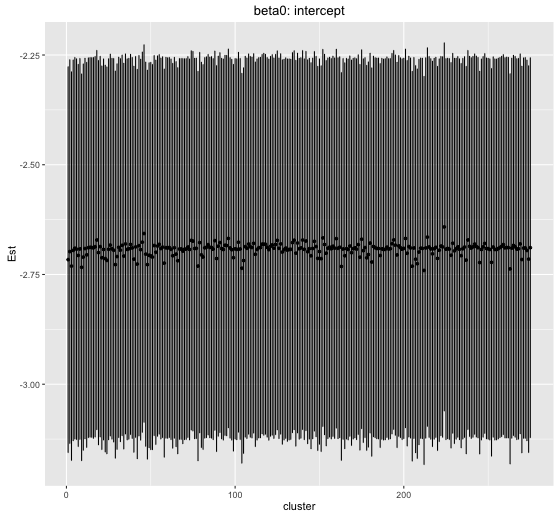
\includegraphics[scale=0.8]{Rplot04-0}
%		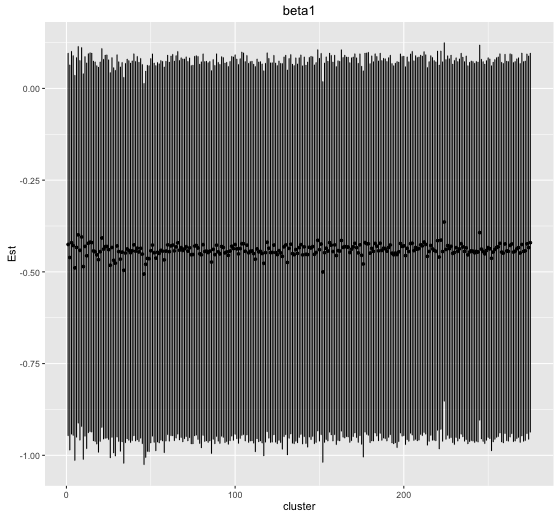
\includegraphics[scale=0.8]{Rplot04-1}
%		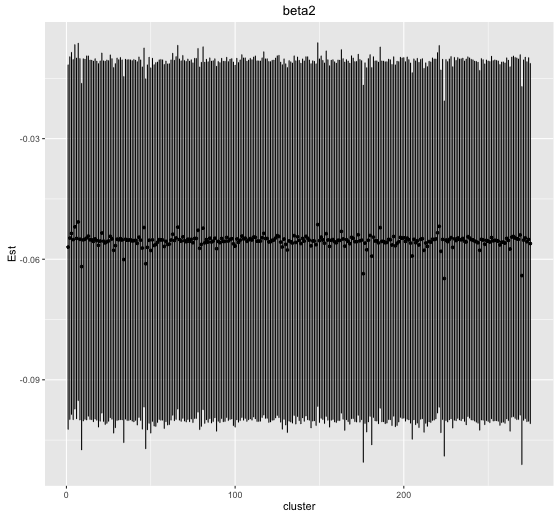
\includegraphics[scale=0.8]{Rplot04-2}
%		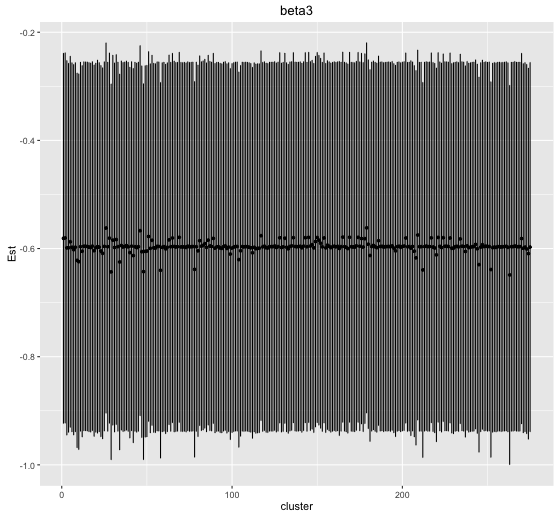
\includegraphics[scale=0.8]{Rplot04-3}
%		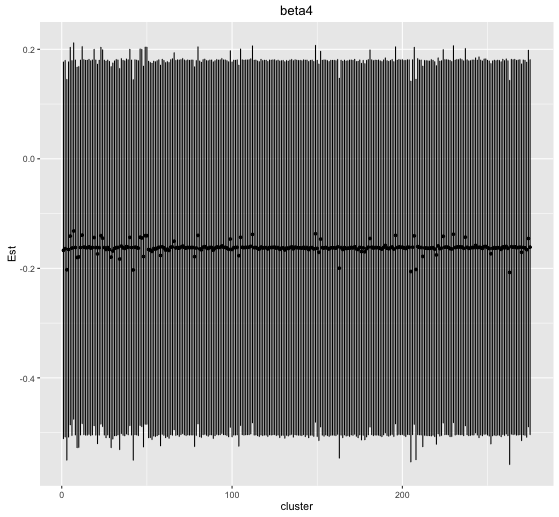
\includegraphics[scale=0.8]{Rplot04-4}
%		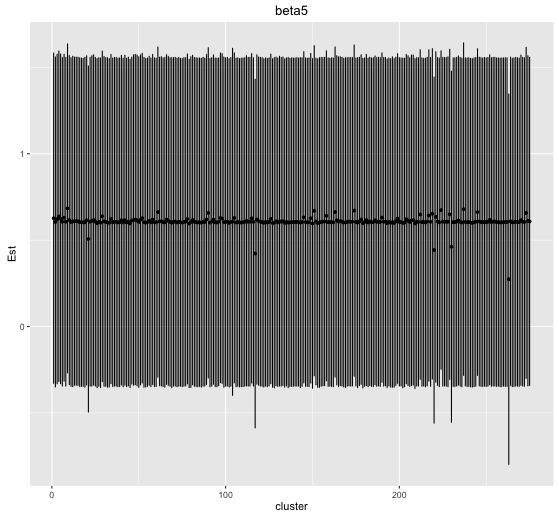
\includegraphics[scale=0.8]{Rplot04-5}
%		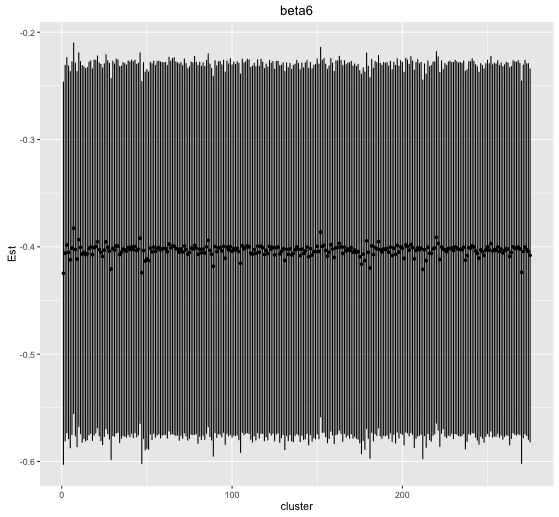
\includegraphics[scale=0.8]{Rplot04-6}	
%	\end{figure}

	\begin{figure}[H]
		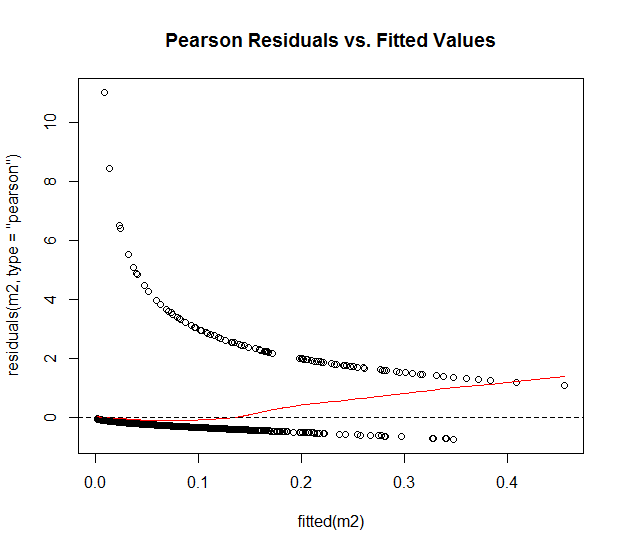
\includegraphics[scale=0.4]{Rplot4-mean1}
		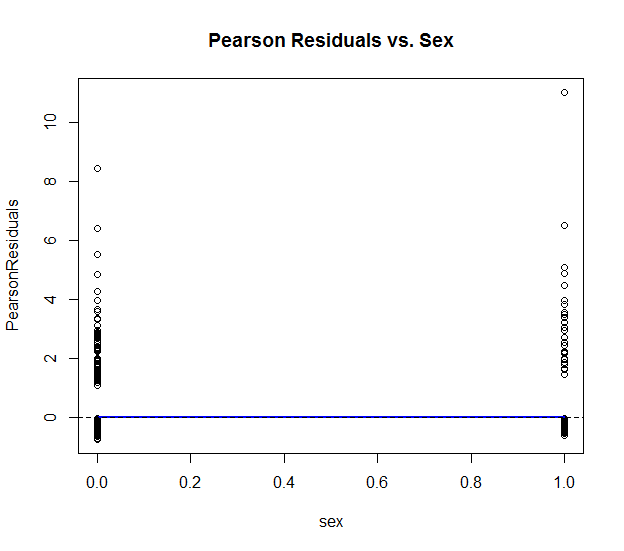
\includegraphics[scale=0.4]{Rplot4-mean2}
		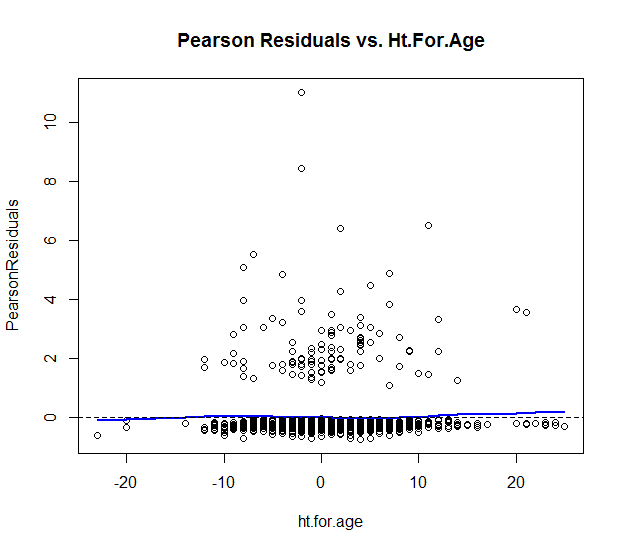
\includegraphics[scale=0.4]{Rplot4-mean3}
		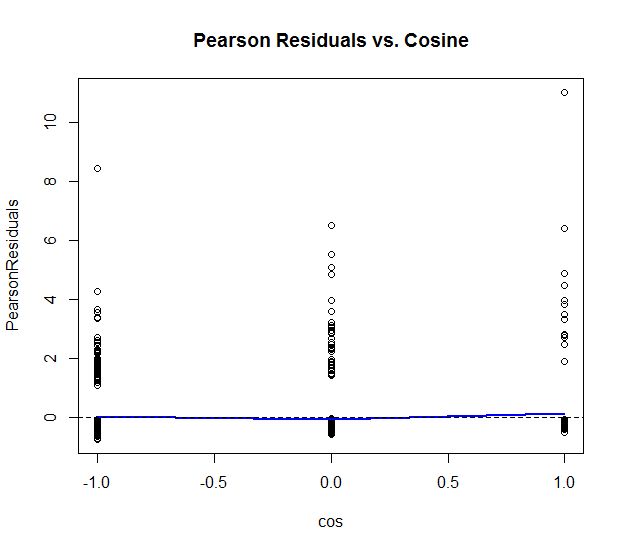
\includegraphics[scale=0.4]{Rplot4-mean4}
	\end{figure}
	\clearpage
	\begin{figure}[H]
		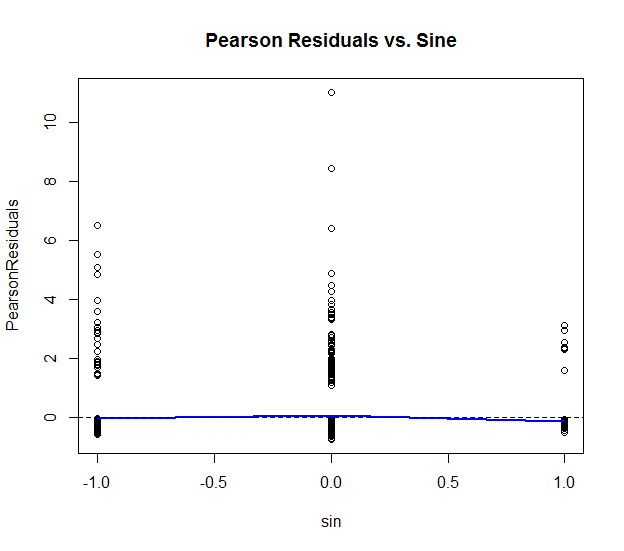
\includegraphics[scale=0.4]{Rplot4-mean5}
		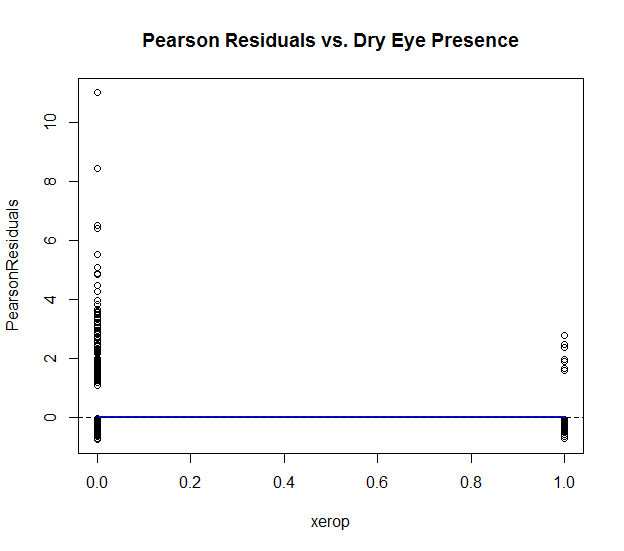
\includegraphics[scale=0.4]{Rplot4-mean6}
		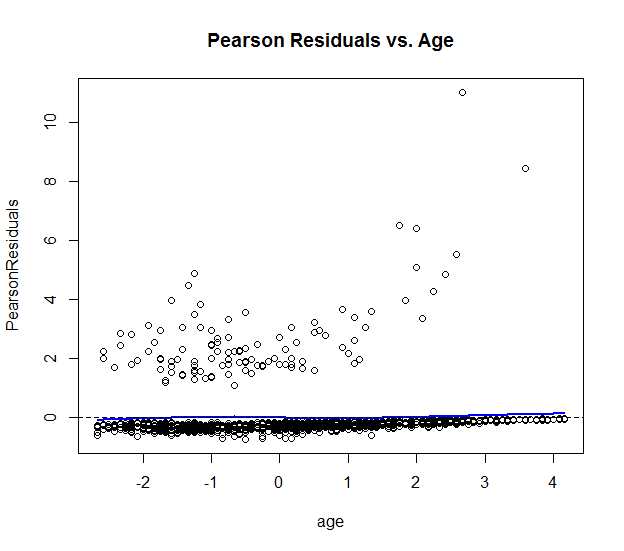
\includegraphics[scale=0.4]{Rplot4-mean7}
		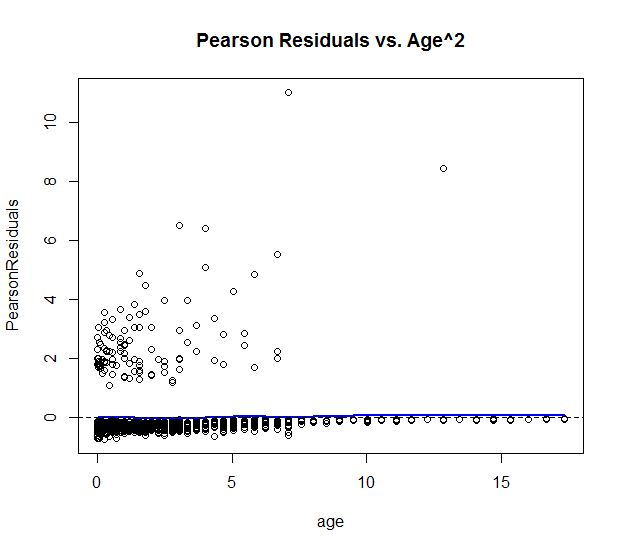
\includegraphics[scale=0.4]{Rplot4-mean8}
	\end{figure}
	There does not appear to be any obvious violations of the residuals on the covariates, but there does appear to be violation of the mean model against the fitted values, where larger fitted values tend to appear with larger Pearson residuals. This is pretty worrisome to me. I think we need to reexamine the mean model, since we might have misspecified it to a pretty serious degree.
\end{enumerate}
\newpage
R code
\begin{verbatim}
	library(geeM)
library(arm)
library(ggplot2)
library(texreg)
library("lme4") # contains the (balanced) sleepstudy data
sleepstudy$DaysC <- with(sleepstudy, Days - mean(Days)) # centering
library("nlme")
lm0c <- lm( Reaction ~ DaysC, sleepstudy) # ignore clustering
lme1 <- lme(Reaction ~ DaysC, random=~1|Subject, data=sleepstudy)
lme2a <- lme(Reaction ~ DaysC, random=reStruct(~DaysC|Subject, pdClass="pdDiag"),
             data=sleepstudy) # diagonal G
lme2b <- lme(Reaction ~ DaysC, random=~DaysC|Subject,
             data=sleepstudy) # unrestricted G
yMarg <- fitted(lme2a, level=0)[1:10] #marginal means, just need to grab the first 10
#need Sigma_i = ziGzi^T + phi R_i now...
VarCorr(lme2a)
z = model.matrix(lme2a,data=sleepstudy)[1:10,] #need these rows for the z_i
G = diag(
  VarCorr(lme2a)[1:2,1]
)
#correlation DEFAULTS to null, so no correlation, so R_i = I
Sig = z%*%G%*%t(z) + diag(VarCorr(lme2a)[3,1],nrow=10,ncol=10)
ses = sqrt(diag(Sig))


upper = yMarg + 1.96*ses
lower = yMarg - 1.96*ses
plot(yMarg, ylim=c(100,500), main="Marignal Mean and 95% Confidence Intervals, Centered X")
for(i in 1:10)
{
  segments(x0=i,y0=lower[i],x1=i,y1=upper[i])
}

######now do it without centering, U is for uncentered!
lme2c <- lme(Reaction ~ Days, random=reStruct(~Days|Subject, pdClass="pdDiag"),
             data=sleepstudy) # diagonal G
yMargU <- fitted(lme2c, level=0)[1:10] #marginal means, just need to grab the first 10

zU = model.matrix(lme2c,data=sleepstudy)[1:10,] #need these rows for the z_i
GU = diag(
  VarCorr(lme2c)[1:2,1]
)
#correlation DEFAULTS to null, so no correlation, so R_i = I
SigU = zU%*%GU%*%t(zU) + diag(VarCorr(lme2c)[3,1],nrow=10,ncol=10)
sesU = sqrt(diag(SigU))


upperU = yMargU + 1.96*sesU
lowerU = yMargU - 1.96*sesU

plot(yMargU, ylim=c(100,500), main="Marignal Mean and 95% Confidence Intervals, Uncentered X")
for(i in 1:10)
{
  segments(x0=i,y0=lowerU[i],x1=i,y1=upperU[i])
}  
###########
#problem 2#
###########
n = 10^3
ni = 5
sigb = 1
sigy = 6
b = rnorm(1000,mean=0,sd=sigb)
do.one <- function(n)
{
  y = c()
  for(i in 1:n)
  {
    yi <- rnorm(ni, mean=b[i], sd = sigy) 
    y = append(y,yi)
  }
  mydat = data.frame(y=y,id=rep(1:n,each=ni))
  m1 <- lmer(y ~ 1|id, data=mydat)
  si = se.ranef(m1)$id #same for all, just grab first
  bi = ranef(m1)$id
  lower = bi - 1.96*si
  upper = bi + 1.96*si
  return(mean((lower < b) & (b < upper)))
}

P = replicate(10^4, do.one(10^3))
##################
#problems 3 and 4#
##################
setwd("~/Dropbox/UW2015-2016/Win2016/571/hw8")
setwd("C:\\Users\\aengl_000\\Dropbox\\UW2015-2016\\Win2016\\571\\hw8")
dat <- read.table("xerop.csv", sep=",", header=T)

dat$cos <- cos(0.5*pi*(dat$time+1))
dat$sin <- sin(0.5*pi*(dat$time+1))

m1 <- geem(respinfect ~ sex + ht.for.age  + cos + sin + xerop + poly(age,degree=2,raw=T), family=binomial, corstr="ar1", data=dat, id=id)

m2 <- glmer(respinfect ~ (1|id) + sex + ht.for.age  + cos + sin + xerop +  poly(age,degree=2,raw=T), family=binomial, data=dat, start=list(fixef = m1$beta))
m3 <- glmer(respinfect ~ (1|id) + sex + ht.for.age  + cos + sin  +  poly(age,degree=2,raw=T), family=binomial, data=dat)
xtable(anova(m3,m2))


#subject-level fitted values against subject-level pearson residuals (level 1 in both cases)
plot(fitted(m2), residuals(m2, type="pearson"),ylab="PearsonResiduals",xlab="Fitted Values", main="Pearson Residuals vs. Fitted Values")
lines(lowess(fitted(m2),residuals(m2,type="pearson"),iter=0),col="red")
abline(h=0, lty=2)

#Pearson Residuals vs. sex, ht.for.age, cos, sin, xerop, age
plot(dat$sex,residuals(m2,type="pearson"),ylab="PearsonResiduals",xlab="sex", main="Pearson Residuals vs. Sex")
lines(lowess(dat$sex,residuals(m2,type="pearson"),iter=0),col="blue",lwd=2)
abline(h=0, lty=2)

plot(dat$ht.for.age,residuals(m2,type="pearson"),ylab="PearsonResiduals",xlab="ht.for.age", main="Pearson Residuals vs. Ht.For.Age")
lines(lowess(dat$ht.for.age,residuals(m2,type="pearson"),iter=0),col="blue",lwd=2)
abline(h=0, lty=2)

plot(dat$cos,residuals(m2,type="pearson"),ylab="PearsonResiduals",xlab="cos", main="Pearson Residuals vs. Cosine")
lines(lowess(dat$cos,residuals(m2,type="pearson"),iter=0),col="blue",lwd=2)
abline(h=0,lty=2)

plot(dat$sin,residuals(m2,type="pearson"),ylab="PearsonResiduals",xlab="sin",main="Pearson Residuals vs. Sine")
lines(lowess(dat$sin,residuals(m2,type="pearson"),iter=0),col="blue",lwd=2)
abline(h=0, lty=2)

plot(dat$xerop,residuals(m2,type="pearson"),ylab="PearsonResiduals",xlab="xerop", main="Pearson Residuals vs. Dry Eye Presence")
lines(lowess(dat$xerop,residuals(m2,type="pearson"),iter=0),col="blue",lwd=2)
abline(h=0, lty=2)

plot(dat$age,residuals(m2,type="pearson"),ylab="PearsonResiduals",xlab="age", main="Pearson Residuals vs. Age")
lines(lowess(dat$age,residuals(m2,type="pearson"),iter=0),col="blue",lwd=2)
abline(h=0, lty=2)

plot(dat$age^2,residuals(m2,type="pearson"),ylab="PearsonResiduals",xlab="age", main="Pearson Residuals vs. Age^2")
lines(lowess(dat$age^2,residuals(m2,type="pearson"),iter=0),col="blue",lwd=2)
abline(h=0, lty=2)

\end{verbatim}
\end{document}



